\documentclass[10pt]{article}
\usepackage{icmlko}

\icmlmeta{IP 파운데이션 월드모델}{323}{답은 내 노트에 있었다}{노트 322 의 전제가 틀렸다 --- 검사는 셋을 정확히 갈랐고, 내가 확인을 안 했을 뿐이다}

\begin{document}

\twocolumn[
\icmlheader

\begin{abstract}
노트 322가 ``\texttt{fund\_cat} 과 \texttt{mkt\_cat} 이 \textbf{검사 ①②③④
를 둘 다 통과}하는데 이득이 스무 배 다르다''를 전제로 ``검사는 거르지 줄
세우지 못한다''를 결론냈다. \textbf{전제가 틀렸다.} 도구를 불러 확인하니
\texttt{mkt\_cat} 은 \textbf{검사 ③ 에서 떨어진다} --- 공유 축을 통제하면
$p{=}0.0941$ 로 ``\textbf{이미 있다}''이고, 검사 ② 는 20건 이상 무리가
\textbf{0개}라 애초에 못 돌린다. 셋을 제대로 세우면 이렇다:
\textbf{\texttt{fund\_cat} 은 넷을 다 통과하고 $+$0.1173 을 번다} ·
\texttt{mkt\_cat} 은 ③ 에서 떨어지고 $+$0.0259 · \texttt{anime\_medium} 은
④ 에서 떨어지고 $-$0.0091. \textbf{검사 넷이 셋을 정확히 갈랐다} ---
떨어진 둘이 \emph{서로 다른} 검사에서 떨어졌고 둘 다 못 벌었다.
\textbf{그래서 노트 322의 표제를 무른다.} 그리고 어떻게 틀렸는지가 더
중요하다 --- \textbf{답이 내 노트에 두 번 적혀 있었다.} 노트 299가 ``시장팝업
category 는 공유 축을 통제하면 안 남는다($p{=}0.1176$)''로 끝났고, 노트 300의
판 전체 감사표에 \texttt{mkt\_cat} 이 ``이미 있다''로 올라 있다. 그리고
\texttt{lab/overlap.py} 는 부르면 0.3초에 답한다. \textbf{쓴 사람도 나이고
도구를 만든 사람도 나인데 안 불렀다.}
\end{abstract}
]

\section{전제를 확인했다}

노트 322의 첫 문장이 ``검사 ①②③④ 를 둘 다 통과하고''였다. 그 문장을
\textbf{안 재고 썼다.} \texttt{lab/overlap.py} 를 불렀다.

\begin{figure*}[t]
\centering
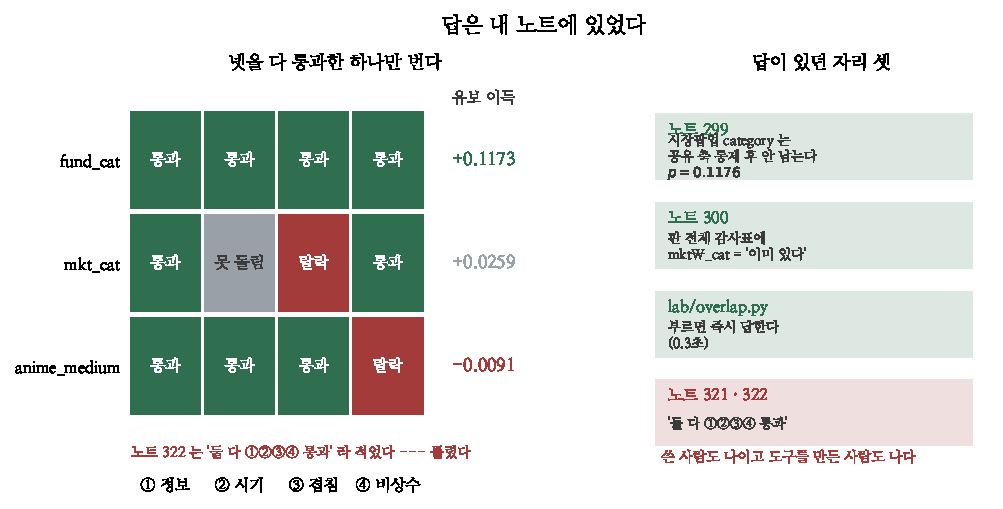
\includegraphics[width=\textwidth]{figs/matrix.pdf}
\caption{왼쪽 --- 전용 축 셋의 검사 결과와 유보 이득. 오른쪽 --- 답이
있던 자리.}
\end{figure*}

\begin{center}\footnotesize
\begin{tabular}{lrrl}
\hline
축 & 혼자 & 통제 후 & 판정 \\
\hline
\texttt{fund\_cat} & $p{<}$1e-4 & $p{=}0.0002$ & \textbf{새롭다} \\
\texttt{mkt\_cat} & $p{=}0.0054$ & \textbf{$p{=}0.0941$} & \textbf{이미 있다} \\
\texttt{anime\_medium} & $p{=}0.0123$ & $p{<}$1e-4 & 새롭다 \\
\hline
\end{tabular}
\end{center}

\textbf{\texttt{mkt\_cat} 은 검사 ③ 에서 떨어진다.} 그리고 검사 ② 도 못
돌린다 --- 시장팝업 학습 101행에 무리 일곱이라 \textbf{20건 이상인 무리가
0개}다(시간 조각 다섯으로 나누면 무리당 서너 행).

\section{제대로 세우면 검사가 갈랐다}

\begin{center}\small
\begin{tabular}{lccccr}
\hline
축 & ① & ② & ③ & ④ & 유보 이득 \\
\hline
\texttt{fund\_cat} & \checkmark & \checkmark & \checkmark & \checkmark
 & \textbf{$+$0.1173} \\
\texttt{mkt\_cat} & \checkmark & --- & \textbf{$\times$} & \checkmark
 & $+$0.0259 \\
\texttt{anime\_medium} & \checkmark & \checkmark & \checkmark
 & \textbf{$\times$} & $-$0.0091 \\
\hline
\end{tabular}
\end{center}

\textbf{넷을 다 통과한 하나만 번다.} 그리고 떨어진 둘이 \emph{서로 다른}
검사에서 떨어졌다 --- \texttt{mkt\_cat} 은 겹침(③), \texttt{anime\_medium}
은 비상수성(④). \textbf{두 검사가 각자 일을 했다.}

\paragraph{노트 322의 표제를 무른다} ``검사는 거르지 줄 세우지 못한다''는
전제가 틀린 결론이다. \textbf{표본 셋에서는 검사가 정확히 갈랐다.}

\begin{center}\footnotesize
\begin{tabular}{ll}
\hline
노트 322에서 & 상태 \\
\hline
``검사는 줄 세우지 못한다'' & \textbf{무른다} \\
몫 가설 반증(가중 $\to$ 안 산다) & \textbf{산다} \\
유보 $\epsilon^2$ 가 거꾸로 & \textbf{산다}(더 이상해졌다) \\
시장 태깅 갈래 닫음 & \textbf{산다} \\
학습 $\epsilon^2$ · 기준 $\rho$ 로 정렬 & \textbf{쓸모없어졌다} \\
\hline
\end{tabular}
\end{center}

마지막 줄이 중요하다 --- 노트 322가 ``어떤 성질이 셋을 정렬하나''를 물었는데
\textbf{애초에 검사가 정렬했으므로 그 물음이 필요 없었다.}

\section{답이 있던 자리 셋}

\begin{center}\footnotesize
\begin{tabular}{ll}
\hline
자리 & 무엇이 적혀 있었나 \\
\hline
\textbf{노트 299} & ``시장팝업 category 는 공유 축을 통제하면 \\
 & 안 남는다'' ($H{=}11.5$, $p{=}0.1176$) \\
\textbf{노트 300} & 판 전체 감사표에 \texttt{mkt\_cat} ``이미 있다'' \\
\textbf{\texttt{overlap.py}} & 부르면 0.3초에 답한다 \\
\hline
\end{tabular}
\end{center}

\textbf{노트 299는 내가 썼고 표제가 ``제일 잘 가르는 것이 이미 판 안에
있었다''였다.} 그 노트의 주인공이 바로 시장팝업 \texttt{category} 다.
\textbf{그리고 노트 300에서 그것을 판 전체 감사표에 올렸다.} 그런데 노트
321에서 축을 훑을 때 ``\texttt{market.category} 이미 있다''를
\emph{선별기의 검증 사례}로만 읽고, 그것이 \emph{배포된 \texttt{mkt\_cat}
그 자체}라는 것을 안 이었다.

\paragraph{왜 안 불렀나} 노트 321 · 322를 쓸 때 관심이 ``새 축을 찾는 것''과
``왜 안 버나''에 있었고, \texttt{mkt\_cat} 은 \emph{이미 아는 것}으로 뒀다.
\textbf{아는 것이라고 생각한 것을 안 쟀다.} 오늘만 두 번째다(노트 306도
``갈래에 적힌 30$\sim$41\%''가 낡은 것을 재다 걸렸다).

\section{그래서 고친다}

\begin{center}\footnotesize
\begin{tabular}{ll}
\hline
고침 & \\
\hline
축을 지을 때 & \texttt{overlap.test3} 결과를 모듈 문서에 박는다 \\
축을 비교할 때 & 검사 넷을 \emph{다시} 부른다 --- 기억을 안 쓴다 \\
\texttt{mkt\_cat} & ``③ 탈락''을 \texttt{mktaxes.py} 에 적는다 \\
\hline
\end{tabular}
\end{center}

\texttt{lab/mktaxes.py} 의 문서에 검사 결과가 없었다 --- 노트 285가 만들 때
③ 이 아직 없었기 때문이다(노트 299가 ③ 을 처음 돌렸다). \textbf{도구가
나중에 생기면 옛 모듈에 소급해 적어야 한다}(노트 306의 규약과 같다).

\paragraph{남은 것}
\begin{center}\small
\begin{tabular}{ll}
\hline
갈래 & 왜 \\
\hline
\texttt{mkt\_cat} 을 뺄까 & ③ 탈락 · $+$0.026 은 문턱 아래 \\
검사 넷을 모듈에 박기 & 기억으로 쓰지 않게 \\
유보 $\epsilon^2$ 가 거꾸로 & 노트 322에서 살아남은 수수께끼 \\
넷째 축을 지어 확인 & 검사가 또 갈리나 \\
\hline
\end{tabular}
\end{center}

\paragraph{규약} \textbf{아는 것이라고 생각한 것을 재라.} 오늘 노트 306이
``갈래에 적힌 숫자가 낡았다''로 시작했고, 노트 314가 ``F18 로 잰 순서가
복제 안 된다''를 봤고, 이 노트가 ``내가 쓴 결론을 내가 안 읽었다''다.
\textbf{셋 다 \emph{새로 재서} 나왔지 생각해서 나오지 않았다.}
그리고 \textbf{도구를 만들었으면 주장할 때마다 부르라} --- 0.3초짜리
호출을 안 해서 노트 하나가 통째로 틀린 전제 위에 섰다.

\end{document}
